\documentclass[main]{subfiles}


\begin{document}
\newpage
\section{Reinforcement Learning}
 Reinforcement learning fuses ideas from neuroscience and AI. The model describes how an agent can interact with an environment and in that environment learn to improve its actions when it comes to gathering a targeted reward. 
 
 
  \begin{figure}[H]
	\centering
	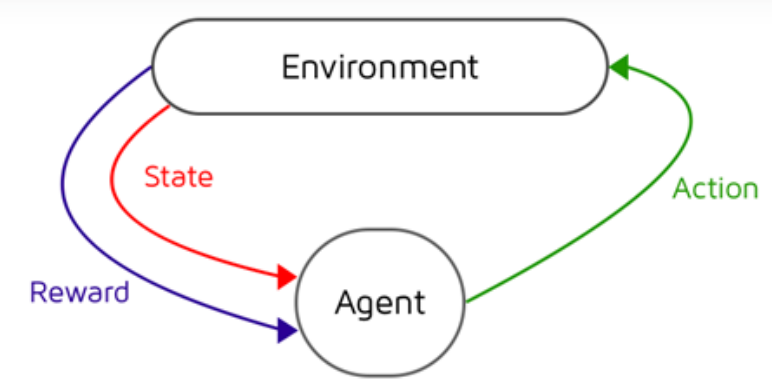
\includegraphics[width=0.9\linewidth]{08_ReinforcementLearning/figures/rl-env-agent-1.png}
	\label{fig:rl-env-agent-1}
	\caption{Connections between an agent and the environment.}
\end{figure}

\begin{itemize}
    \item There is only a reward/supervision signal after each action.
    \item Feedback is often delayed and not instantaneous.
    \item Time needs to be taken into account.
    \item The agent’s actions affect the subsequent data it receives.
\end{itemize}



 \subsection{Dopamine: Reward Prediction Error}
From Schultz (89) \footnote{Predictive Reward Signal of Dopamine Neurons}: Dopamine neurons are activated by rewarding events that are better than predicted, remain uninfluenced by events that are as good as predicted, and are depressed by events that are worse than predicted. Most dopamine nerons show phasic avtivations ... reward-predicting ... However only few phasic activations follow aversive (causing avoidance of a thing) stimuli. By signaling rewards  according to a prediction error, dopamine responses have the formal characteristics of a teaching signal postulated by reinforcement learning theories.
 

  \begin{figure}[H]
	\centering
	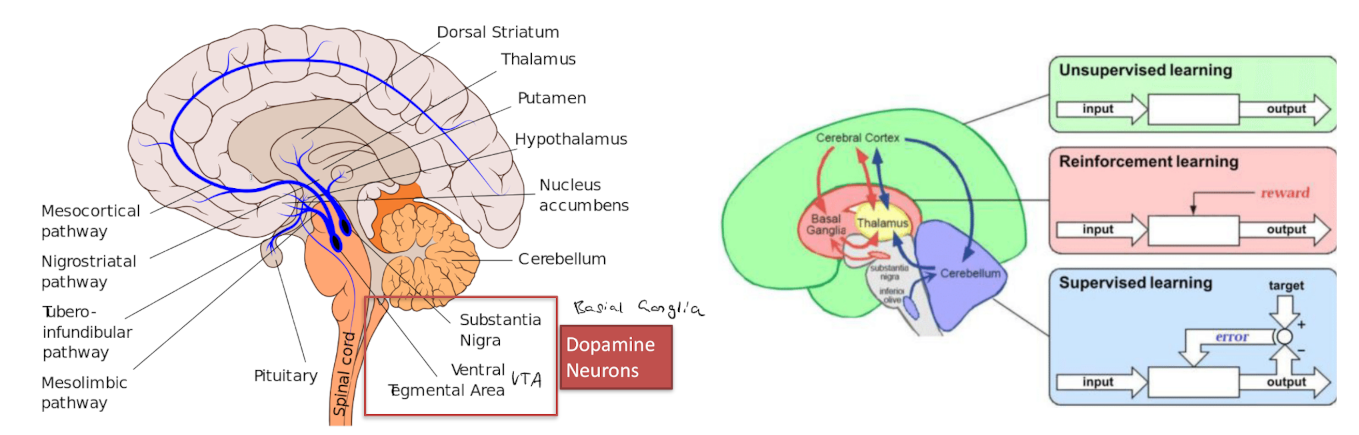
\includegraphics[width=0.9\linewidth]{08_ReinforcementLearning/figures/rl-in-brain.png}
	\label{fig:rl-in-brain}
	\caption{Dopamine neurons of Substantia Nigra and the Ventral Tegmental Area in the Basal Ganglia. (right) Mapping of different machine learning paradigmns to the brain. }
\end{figure}

If the neocortex mostly performs unsupervised learning why does the VTA strongly project to almost all cortical areas and what is the effect of DA on a cortical neuron?

\begin{itemize}
    \item Ventral structure does not project to dorsal (where we assume RL happening).
    \item Gated reinforcement learning: we only want to learn relevant information
    \item Dopamine is connected to plasticity because it is very sensitive to new / unseen data.
\end{itemize}

\begin{figure}[H]
	\centering
	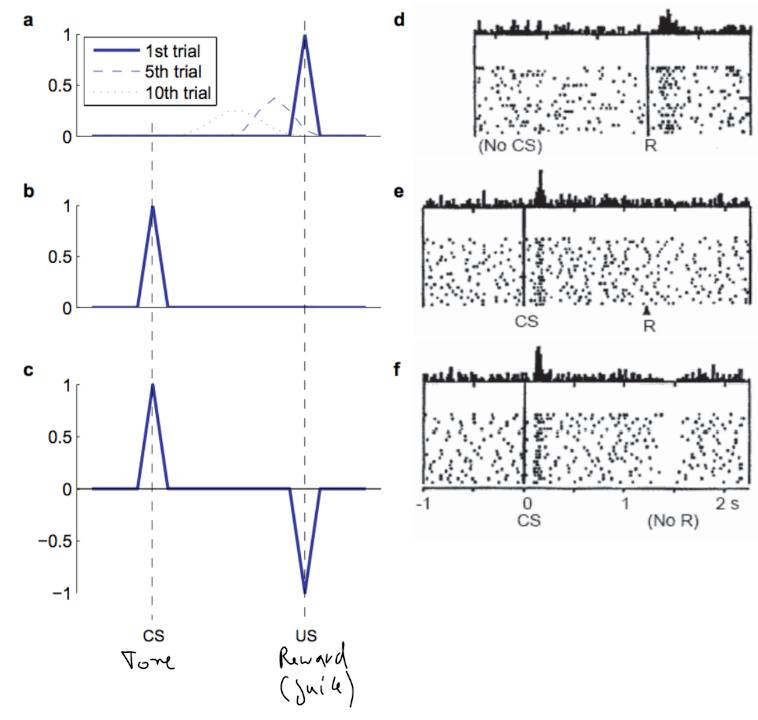
\includegraphics[width=0.9\linewidth]{08_ReinforcementLearning/figures/dopamine-rpe.png}
	\label{fig:dopamine-rpe}
	\caption{ Dopamine neurons report rewards according to an error in reward prediction. Top: drop of liquid occurs although no reward is predicted at this time. Middle: conditioned stimulus predicts a reward, and the reward occurs according to the prediction, hence no error in the prediction of reward. Bottom: conditioned stimulus predicts a reward, but the reward fails to occur because of lack of reaction by the animal.CS, conditioned stimulus; R, primary reward.}
\end{figure}

The predicted reward is further modified by other factors: 

Timing of reward: Across species, it is clear that signals related to predictionerrors are modulated by cues that predict delayed reward. Animals prefer an immediate reward over a delayed reward even when the delayed reward is more economically valuable in the long run. \footnote{Impact of size and delay on neural activity in the rat limbic corticostriatal system}

Adaption to a new situation: We found that midbrain dopamine neurons rapidly adapted to the infirmation provided by reward-predicting stimuli. Responses shifted relative to the expected reward value, and the gain adjusted to the variance of reward value \footnote{Adaptive Coding of Reward Value by Dopamine Neurons}.

\subsection{Models of Reward Prediction}

\subsubsection{Rescorla Wagner Rule}
Model of classical conditioning in which learning is conceptualized in terms of associations between conditioned and unconditioned stimuli. Change in value $V(s_t)$ is proportional to the difference between actual and predicted reward.

\begin{equation}
    V(s_{t}) \leftarrow V(s_t) + \eta[R- V_{total}]
\end{equation}

where:

\begin{itemize}
    \item $s_t$: stimulus
    \item $V(s_t)$: associative strength of conditioned stimulus $s_t$
    \item $R$: reward
    \item $\eta$: learning rate
    \item $V_{total}$ sum of associative strengts of all conditioned stimului (including $s_t$) that are presented on this trial (the n-th trial).
    \item $|[R- V_{total}]|$ surprise
\end{itemize}

\begin{figure}[H]
	\centering
	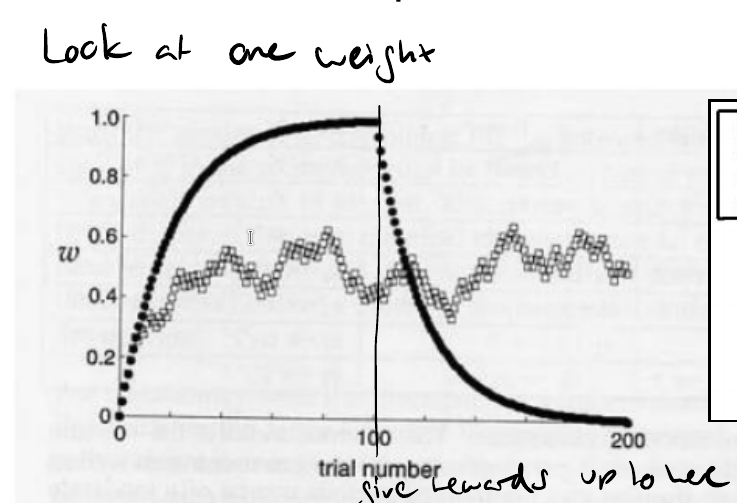
\includegraphics[width=0.9\linewidth]{08_ReinforcementLearning/figures/rw-rule.png}
	\label{fig:rw-rule}
	\caption{Typical exponential / log behavior of the iterative R-W rule.}
\end{figure}


\subsection{Temporal Difference Rule to Q-Learning}
Key Idea of the temporal difference rule (TDR): 
Update the value of the current state based on the immediate reward and the estimated value of the next state. 
Interpretation: we must not look at immediate rewards only but future rewards should be taken into consideration as well on a discounted valuation. 
far we assume that the path that our agent takes to navigate the system is given.


\begin{equation}
    V(s_{t}) \leftarrow V(s_t) + \eta[r_{t+1} + \gamma V(s_{t+1}) - V(s_t) ]
\end{equation}

where:

\begin{itemize}
    \item $V(s_t)$: previous estimate
    \item $r_{t+1}$ next reward
    \item $\gamma V(s_{t+1})$ discounted value on the next step
\end{itemize}

Lets now include the fundamental concept of an action to this equation. This adds one dimension to the value function and gives the agent a choice. This new function is called $Q(x,a)$. 
By just a few trivial steps one can show that the TD rule is used to get the convex combination in the Q-Learning update rule between old and new $Q$ value seen in the literature:

\begin{align}
Q(x,a)& \leftarrow (1-\alpha_t)Q(x,a) + \alpha_t(r+\gamma max_{a'}[Q(x',a')]) \\
Q(x,a)& \leftarrow Q(x,a) - \alpha_t Q(x,a)  + \alpha_t r + \gamma \alpha_t max_{a'}[Q(x',a')] \\
Q(x,a)& \leftarrow Q(x,a) + \alpha_t (r + \gamma max_{a'}[Q(x',a')] - Q(x,a)) \\
Q(x,a)& \leftarrow Q(x,a) + \alpha_t (r + \gamma max_{a'}[Q(x',a') - Q(x,a)])
\end{align}

Given this rule, we can create and update a map over future states and actions. We can optimize w.r.t the action to get an optimal path (policy). The key idea idea is that we do not need to know any transition probabilities to learn (model), we just need an unbiased estimate from our world (sample). We can get these samples by just playing the "game". If we store the actions $a$ and rewards $r$ from these samples, we can directly apply Q-learning. Thus, Q-learning is considered model-free.

Keep in mind that (in the end), the optimal policy can be deducted from the optimal value function $V^*$:

\begin{equation}
    V^*(x) = max_a Q^*(x,a)
\end{equation}


\subsection{Reinforcement Learning}
We saw the concept of looking at expected reward and choosing actions to maximize this reward, but the idea was not well embedded into a generalizing concept. 
Reinforcement learning (RL) exactly puts a name on this framework, which includes Q-Learning as well.
RL is about an agent taking suitable action to maximize reward in a particular situation. 
It is employed by various software and machines to find the best possible behavior or path it should take in a specific situation. 

\begin{figure}[H]
	\centering
	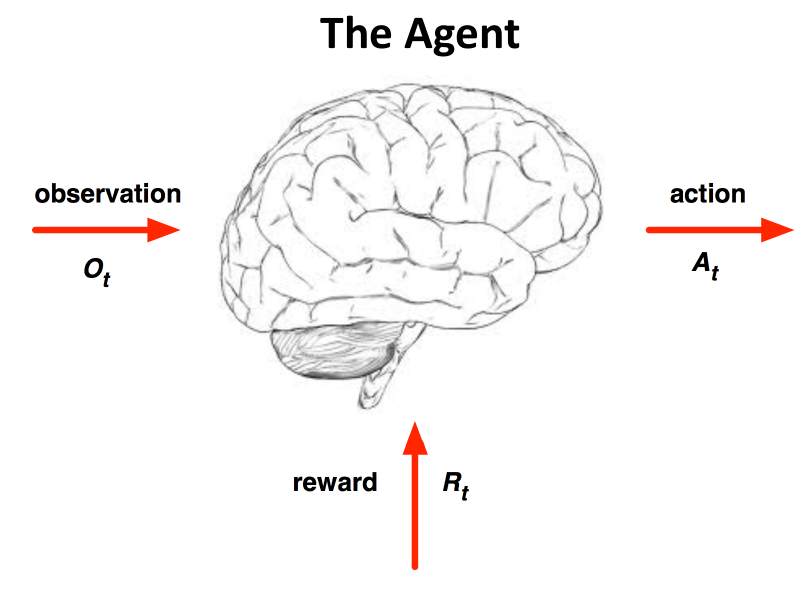
\includegraphics[width=0.9\linewidth]{08_ReinforcementLearning/figures/rl-basic-comps.png}
	\label{fig:rl-basic-comps}
	\caption{Influences from and to the agent in RL to the surrounding world. At each step $t$, the agent exectues an action $A_t$ which the environment recieves. The agent recieves an observation $O_t$ of the environment, for example trough a sensor and the agent is rewarded $R_t$ by its behavior from the environment.}
\end{figure}


Reinforcement learning is based on the reward hypothesis:
\textbf{All goals of an agent can be described by the maximization of expected cumulative reward.}

Example rewards:

\begin{itemize}
    \item Fly stunt maneuvers in an RC helicopter (+ following desired trajectory, - crashing)
    \item Defeat the world champion at Backgammon (+ winning /- loosing)
    \item Manage an investment portfolio (+ more / -  less money)
    \item Make a humanoid robot walk (+ reward for forward motion / − reward for falling over)
    \item Play Atari games better than humans (+/− reward for increasing/decreasing score)
\end{itemize}

The fact that reward presented to the agent is not always immediate leads to the exploration / exploitation dilemma. (Example: A financial investment may take months to mature). 
An agent does not intrinsically know the future implications of its actions, or (how actions interact with) dynamics of the environment.

At each point in time, the agent is in a state. because this information state is all that is necessary to fully determine the agent, it is also said that the state is markovian. This means we can throw away the histrory.

\begin{equation}
    P(S_{t+1}|S_t) = P(S_{t+1} | S_{1:t})
\end{equation}

An RL agent may compute different functions on top of its state.

\subsubsection{Policy}
The agents behavior function callend policy maps from state $s$ to action $a$. The policy may be stochastic or deterministic:

\begin{align}
    a & = \pi(s) \\
    \pi(a|s) & = P(A_t = a | S_t = s)
\end{align}

\subsubsection{Value Function}
Value function is a prediction of future rewards and does so by assigning a number to every state $s$. It depends on a policy $\pi$ to determine where the agent could go and a probability distribution $p(X'|\pi(X), X)$.

We compute this value as expectation over the joint distribution:
\begin{equation}
p(S_{1}, S_{2}, S_{3}, \dots)
\end{equation}

The value function is defined as: 
\begin{equation}
    v_{\pi} = \mathbb{E}[r(s_0, \pi(s_0)) + \gamma r(s_1, \pi(s_1)) + \gamma^2 r(s_2, \pi(s_2)) + \dots]
\end{equation}

But in the  lecture, they mentioned (and it is not distinguished between the two) the conditional value function:

\begin{equation}
    v_{\pi}(s_0) = \mathbb{E}[\sum_{t=0}^\infty \gamma^t r(s_t, \pi(s_t) | S_0 = s_0]
\end{equation}

Which can be rewritten to the recursive equation (often in the literature):
\begin{equation}
v_{\pi}(s) = r(s_0, \pi(s_0)) + \gamma \sum_{s_1} p(S_1 =s_1 | S_0 = s_0)
\end{equation}



\end{document}